\section{System Design}
\label{sec-design}

\subsection{Design Principal}
To solve the challenges and outperform the state-of-the-arts for this new shoulder surfing attack, we propose a holistic system with the multi-frame SR neural network, illustrated in Figure~\ref{fig-workflow}.
%\cl{These four parts are too long, try to whittle it away to half its length. Refer to the revised contents for challenges in Section introduction.}

\begin{itemize}[leftmargin=*]
    \item \textbf{Layered architecture and frequent introduction of input.} To counter the blurriness of the images, and the tendency of reconstructing fake characters, our network is constructed with several identical SR layers, connected sequentially, and the images are refined step by step throughout the layers. All input images are processed simultaneously and separately, with the information from other images for reference, throughout the network. Another importent feature of our architecture is that the initial input images are introduced into the dataflow at each layer, from beginning to end, resulting in the uneven depth of our model, acting as an anchor for the reconstruction process so that the output will be faithful to truth from beginning to end, while preserving the deep mainstream of the model to be able to process such blurry images.
    \item \textbf{Merging layers to adapt multiple frames.} A merging process inside each layer functions as the revenue of communication across images integrates information from all the images into one, the result of which is then stacked with each image for the next convolution. At each layer the image is exposed to the consensuses of features from other images at the same level of complexity, acting as a verification for the hypothetical features extracted from the current image, so that in the training process more audacious features can be learned and proposed without fear of punishment from the final loss, increasing the quality of featuremaps throughout the network.
    \item \textbf{Model Complexity and adaption for variable input.} All the convolutional layers throughout the network are performed individually for each image(or the featuremaps of them from the previous layer), and these convolutions in the same layer share a same set of parameters in training and production, thus reducing parameter count and avoiding convolutions for large numbers of channels, saving calculation power. This trait also enables the  the same network to adapt any number of input images. On one hand, this gives our model the ability to adapt to the uncertainty of the number of avaliable images, providing relatively satisfactory results regardless whether the attacker has ample time photographing the target phone before it changes its display; on the other hand, the relative independence and the isotropy of the merging layers avoids the reliance on sequential order and consistency between neighboring frames(which is common among most multi-frame SR networks), solving the inconsistency problem mentioned in Figure~\ref{illustration_of_system}.
    \item \textbf{Compatibility with complex characters.} The discrete distribution of characters leads to the inclination of diviation and producing 'fake' results. The frequent introduction of input images is designed to mitigate this challenge. Also, our model can learn correlations between certain features and strokes from the training data, decomposing the SR problem and making it a lot less challenging. We also introduce adaptive boosting\cite{adaboost} in our training process, increasing the loss weight of the wrongly reconstructed characters, determined by loss in earlier stages and OCR in later stages, to accommodate the imbalanceness of data. The loss functions in training is also redesigned. The mean square error(MSE) is not suitable in this application, as a misplaced stroke, although highly obstructing readability, may only invoke a slight decrease in MSE because it only influenced a few pixels. Our solution is putting a weight on each pixel before applying weighted MSE. Assuming the characters are black on white, this weight increases at darker pixels and propagates to neighbouring dark pixels so that long strokes and intersections of strokes are given higher weights. This process serves as a supplement to MSE to focus more on readability and is beneficial for OCR and human reading tests. 
  \end{itemize}

\subsection{Network Design}
The core of the \textsf{SRPeek} system is a specially designed multi-frame SR neural network, accepting a group of $N$ images indexed $x_1^{(0)}$ to $x_N^{(0)}$ as input and generating an image with higher resolution $y$ as output. The network comprises $L$ layers, each of which implements a non-linear transformation $H_l(\cdot)$, where $l$ indexes the layer. As mentioned before, in each layer images are processed separately, with the merging layers as a revenue for communication, so that the output of each layer is correspondent to the input.  We denote the output of the $l^{th}$ layer as $x_1^{(l)}$ to $x_N^{(l)}$, which is also the input of the $(l+1)^{th}$ layer. Till now the model is not different from traditional SR models:
\begin{equation}\label{eq:1}
    \begin{split}
x_i^{(l)} = H_l(x_i^{(l-1)}), i=1,2,...N
\end{split}
\end{equation}

%\cl{function above cannot express merging between x1 x2 ... xN?}

Additionally, we introduce the initial images $x_i^{(0)}$ as an input for all the layers:
\begin{equation}\label{eq:2}
    \begin{split}
        x_i^{(l)} = H_l(x_i^{(l-1)},x_i^{(0)}), i=1,2,...N
\end{split}
\end{equation}

The last layer is exceptional, it yields a single image $y$ as output. 

Presently, in these layers nothing is done to raise the resolution of the images, so that the resolution of $x_i^{(0)}$ to $x_i^{(l-1)}$ and $y$ remains the same. To increase resolution we insert several 2$\times$ nearest upsampling layers $U$ evenly throughout the architecture between the layers:
\begin{equation}\label{eq:3}
    \begin{split}
        x_i^{(l)} \leftarrow U(x_i^{(l)}), x_i^{(0)} \leftarrow U(x_i^{(0)}), i=1,2,...N
\end{split}
\end{equation}

we upsample the input images $x_i^{(0)}$ simultaneously to keep the two inputs of the following layers $H_l(x_i^{(l-1)},x_i^{(0)})$ unanimous in resolution. For example, in a 4$\times$ SR network with five layers, we may insert 2 2$\times$ nearest upsampling layers behind the 2nd and 4th layer.

Inside each layer $H_l$ there are 3 convolution layers $Conv_{1l}(\cdot)$, $Conv_{2l}(\cdot)$, $Conv_{3l}(\cdot)$ and 1 merging layer $Merge_l(\cdot)$.

%\cl{$H(\cdot)$ or $H(\cdot,\cdot)$?}
\begin{figure}
    \centering
       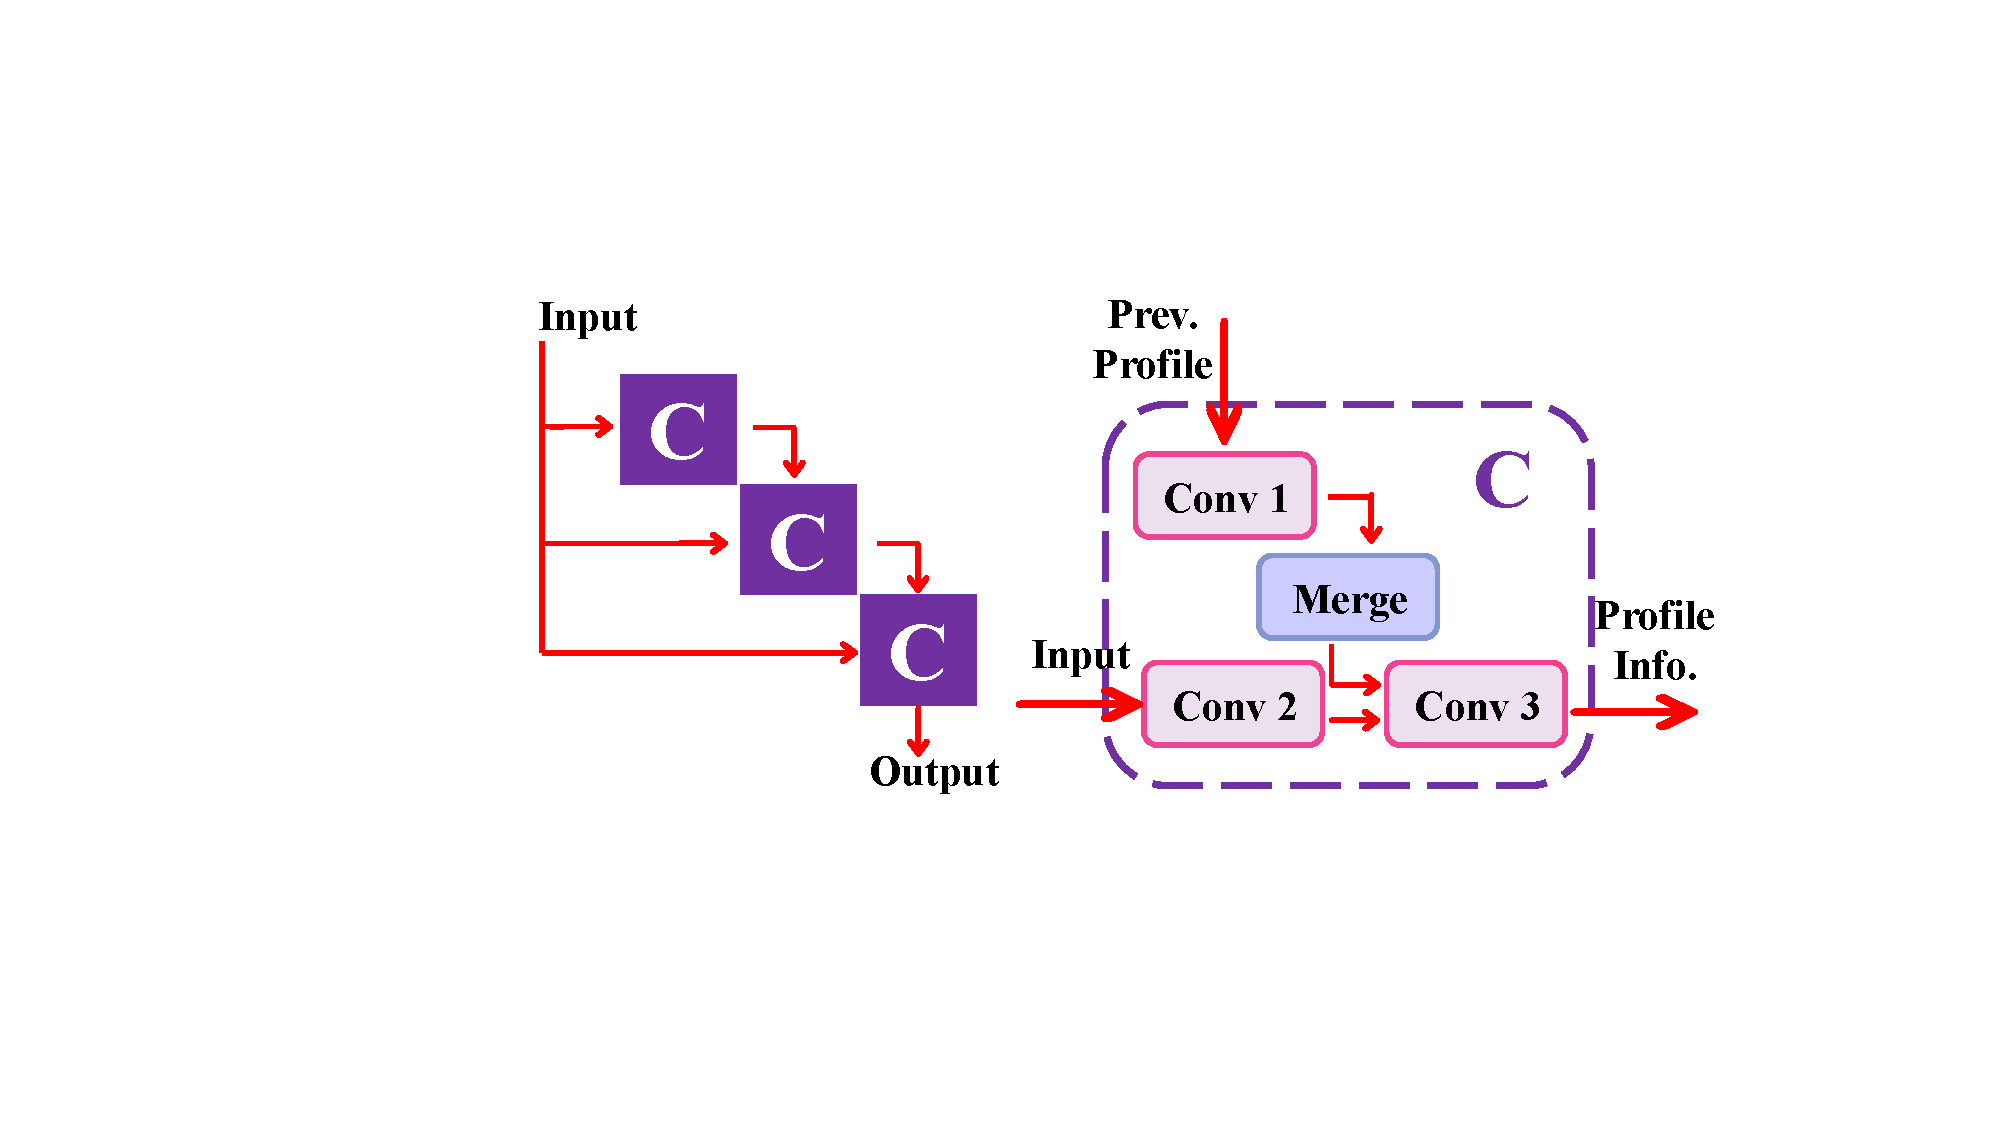
\includegraphics[width=0.5\textwidth]{./pic/network.pdf}
       \caption{Network Architecture of SRPeek.}
       \label{fig-system}
   \end{figure}   

\vspace{1mm}
\noindent
\textbf{Conv1:} The first convolutional layer, $Conv1$, accepts the layer's first input parameter $x_i^{(l-1)}$ as input. Note that all three convolutional layers accept a single image(or its featuremaps from the last convolutional layer) as input, the convolutional process is repeated for all the images, and calculations within the same convolutional layer share the same group of parameters all the time (parameters denoted as $Param_{sl}$ for convolutional layer $Conv_{sl}, s=1,2,3$):
\begin{equation}\label{eq:4}
    \begin{split}
        a_i^{(l)} = Conv_{1l}(x_i^{(l-1)},Param_{1l}), i=1,2,...N
\end{split}
\end{equation}

\vspace{1mm}
\noindent
\textbf{Merge:} The results of the previous step of all the images $\{a_1^{(l)},a_2^{(l)},...,a_n^{(l)}\}$ are then passed to the merging layer $Merge_l$ to generate $t$ groups of featuremaps. Suppose the results of $Conv_{1l}$ consists of $R$ channels:
\begin{equation}\label{eq:5}
    \begin{split}
        a_i^{(l)} = \{a_{i1}^{(l)},a_{i2}^{(l)},...,a_{iR}^{(l)}\}, i=1,2,...N
\end{split}
\end{equation}

The data in each channel will be merged separately in the merging layer. The output is $T\times R$ channels, denoted as $b_{tr}^{(l)}(t=1,2,...T, r=1,2,...R)$:

\begin{equation}\label{eq:6}
    \begin{split}
        b_{tr(p,q)}^{(l)} = \sum_{i=1}^{N} a_{ir(p,q)}^{(l)} e^{k_t a_{ir(p,q)}^{(l)}} /\sum e^{k_t a_{ir(p,q)}^{(l)}}
\end{split}
\end{equation}

where (p,q) represent the pixel at this coordinate, and $k_t$ is a set of fixed parameters shared in all the merging layers throughout the model, controlling the behavior of the merging process. Apparently, k=0 leads to averaging, k=${+\infty}$ leads to max operator and k=${-\infty}$ leads to min operator. We use T=5 and k=-1,-0.5,0,0.5,1 in our model, giving consideration to both consensuses (k=0,averaging) and prominent features(k=1, 'soft'max and k=-1, 'soft'min). these $T\times R$ channels $b_{tr}^{(l)}$ is the output of this merging layer $Merge_l$.

\vspace{1mm}
\noindent
\textbf{Conv2:} $Conv2$ is a replica of $Conv1$, processing the layer's second input parameter $x_i^{(0)}$, also generating $N$ outputs with $R$ channels per output, denoted as $c_ir^{(l)}, i=1,2,...N, r=1,2,...R$:
\begin{equation}\label{eq:7}
    \begin{split}
        c_i^{(l)} &= Conv_{2l}(x_i^{(0)},Param_{2l}), i=1,2,...N\\
        c_i^{(l)} &= \{c_{i1}^{(l)},c_{i2}^{(l)},...,c_{iR}^{(l)}\}, i=1,2,...N\\
\end{split}
\end{equation}

\vspace{1mm}
\noindent
\textbf{Conv3:} The data from $Merge$ and $Conv2$ are merged together, in that all the $T\times R$ channels of $b_{tr}^{(l)}$ are replicated N times and stacked with each one of the N outputs of $Conv_{2l}$, before these N outputs, each with $(T+1)\times R$ channels, are passed through the third convolutional layer $Conv_{3l}$. There are also N output of this convolutional layer, denoted as $d_i^{(l)}, i=1,2,...N$:
\begin{equation}\label{eq:8}
    \begin{split}
        d_i^{(l)} = Conv_{3l}(Stack(c_i^{(l)},b^{(l)}),Param_{3l}), i=1,2,...N 
\end{split}
\end{equation}

\vspace{1mm}
\noindent
\textbf{Output:} If $l < L$, this is not the last layer, the N outputs of step (4) will be the output of layer $H_l$. Otherwise, as we need to present a single image $y$ as output, we add another merging and a common convolutional layer after $Conv_{3l}$. The merging layer is identical to the previous $Merge_l$, merging the N outputs $d_i^{(l)}$ into $T\times R$ channels $e_{tr}^{(l)}$, and a convolutional layer processes this $e_{tr}^{(l)}$ to generate a single channel of output $y$. 
\begin{equation}\label{eq:7}
    \begin{split}
        \{e_{tr}^{(L)},t\le T,r\le R\} &= Merge'_{L}(\{d_i^{(L)},i\le N\})\\
        y &= Conv'_{L}(\{e_{tr}^{(L)},t\le T,r\le R\} )\\
\end{split}
\end{equation}

The full structure of a 3 layer network is shown in Figure~\ref{fig-system}.

% \subsection{Design Principal}
% To solve the challenges and outperform the state-of-the-arts for this new shoulder surfing attack, we propose a holistic system with the multi-frame SR neural network, illustrated in Figure~\ref{fig-workflow}.
% \cl{These four parts are too long, try to whittle it away to half its length. Refer to the revised contents for challenges in Section introduction.}

% \subsection{system design}
% We implemented a holistic system for shoulder surfing, with the neural network as core, on a smartphone to verify the efficiency of our model. It iterates through the following steps: 

% \vspace{1mm}
% \noindent
% \textbf{Input:} Under guidance of the attacker, The smartphone will zoom in, take focus, and take 20 images with burst mode of the target screen. Note that the zoom in step is only for easier interaction and focusing, and to utilize the telephoto lenses and optical zoom, if avaliable, as digital zooming do not put in any extra data; On traditional phones with only digital zooming, the photo-taking will be with 1x zoom, and on phones with optical zooming, 5x to 10x zoom, depending on the optical zooming range. This way information on the images will be more compact and easier to comprehend by neural networks.

% \vspace{1mm}
% \noindent
% \textbf{Alignment:} The images are then aligned to mitigate the shifts between frames caused by hand tremor or movements from the lenses, as cameras with optical lenses will ocationally shift slightly across time due to the movements of its inner mechanism. Luckily, in our scenario the target is a glowing screen whose edges are easily distinguishable in most cases, and we use them as reference to align our images. The images are also spun to make the text horizontal in the process. The screen is cropped out and the rest of the image abandoned.


% \vspace{1mm}
% \noindent
% \textbf{Adjustment:} The lines of text(or stuff differing from the background color of the screen) will be carved out for processing, to reduce the workload of the network. The characters are normally around 10x10 pixels in the photos, and the carved segments will leave 2 pixels of padding on all sides to avoid mutilating the character; A certain amount of error is allowed, but if the size of the text is too small or too large, the neural network will not be able to extract features normally, so the images will be zoomed to the right size(and the zooming of step (1) will be adjusted accordingly).


% \vspace{1mm}
% \noindent
% \textbf{Processing:} As our network accepts only 9x9 patches, we will process all the 9x9 patches among the input photo and merge the results together. After carving a 9x9 patch at corresponding locations of each image, these patches are then processed by our multi-frame super resolution network, generating a single 36x36 image (4x upscaling). The input is RGB colored, while the output, as we are not interested in color, is black and white. When all patches are processed, their outputs are merged together. The overlapping pixels are thus processed: among all the outputs containing this pixel, we collect these values, remove outliers, and use their average as the result. In this way, we generate upscaled image segments of all the characters on the target screen, which are then inserted in one of the input images(roughly upscaled to encompass them, just for reference) and displayed to the attacker.

% These steps are repeatedly executed to enable the attacker to monitor the victim at an interval of a few seconds. At critical times requiring continuous monitoring so as not to miss transient display, e.g. password entering, the system can simply lengthen the input phase across that period and process the data afterwards. The workflow of our system is shown in Figure~\ref{fig-workflow}.

